\documentclass[11pt]{article}
\usepackage[margin=1in]{geometry}
\usepackage{booktabs,graphicx,amsmath,hyperref,microtype,enumitem,caption,array}
\usepackage{xcolor}
\hypersetup{colorlinks=true,linkcolor=blue!50!black,urlcolor=blue!50!black,citecolor=blue!50!black}
\setlist{itemsep=2pt,topsep=3pt}
\emergencystretch=3em
\title{\bfseries Tool Use, Not Scale, Decides Small-Model Accuracy\\on Construction Calculation Tasks\\[2pt]\large Evidence from ConstructBench, a Seeded Benchmark with Computed Answers}
\author{Constructelligence Research}
\date{\small Working paper, November 2026 --- not peer reviewed}
\begin{document}
\maketitle
\begin{abstract}\noindent
Construction work is full of procedural arithmetic: schedule calendars, pay-application certification, work-in-progress schedules, delay analysis, bid levelling. A model that reads the right clause can still slip across a hundred ledger rows, or run out of output budget while calculating by hand. We ask whether a sandboxed Python tool and a strict answer schema change accuracy on such tasks, and for which models. We built ConstructBench, a seeded generator suite (17 domains, 58 families) whose reference answers are computed by code and re-derived independently from the prompt text, and compared one identical harness against a no-tools baseline on 84 expert-tier tasks. For a cheap open-weight model (ling-3.0-flash), strict accuracy rose from 40.5\% to 96.4\% (+56.0 points, paired 95\% CI +45.2 to +66.7; 48 tasks better, 1 worse). For Claude Haiku 5.5 it rose from 92.7\% to 100\% on the 82 tasks answered in both conditions (+7.3 points, CI +2.4 to +13.4, $p=0.031$). For DeepSeek Flash the gain (+4.8 points) was not significant. Most of the open-weight gain is completion rather than correctness: 40 of ling's 50 baseline misses were ``no answer'', not wrong numbers. On easier sets the three Claude 5.5 models were already at ceiling and the harness changed cost and latency, not accuracy. We also report a design failure of our own: an attempt to make one task family harder made it easier.
\end{abstract}

\section{Introduction}
Public construction benchmarks are mostly question answering or document retrieval. The failures practitioners report with language models are different: the model finds the right clause and then makes an arithmetic or bookkeeping slip, or exhausts its output budget reasoning in prose. That is as much a tools question as a model question, and it matters for cost, because a small model with a calculator may replace a large one without it. Our contributions:
\begin{enumerate}
\item \textbf{ConstructBench}: open-ended generators with computed answers, per-field tolerances, an independent second implementation of every expert-tier answer, and decontamination tooling.
\item A \textbf{single tool harness}, identical across Anthropic and OpenAI-compatible APIs, so conditions differ only in tools.
\item A \textbf{paired, pre-registered analysis} of harness against no harness, with failure categories.
\item A \textbf{reporting policy} separating completion, format compliance and strict accuracy, because one accuracy figure conflated all three in our own early runs (Section~\ref{sec:method-findings}).
\end{enumerate}

\section{ConstructBench}
Tasks come from seeded Python generators; a set is fixed by its seed and per-family count. Answers are computed by the generator, never keyed by hand, and every prompt states every convention so that exactly one answer is correct. Domains include architecture, estimating, preconstruction, scheduling, project management, finance, contracts and claims, civil, quality, safety, sustainability, real estate, BIM and robotics, at five tiers (easy, medium, hard, expert, extreme).

\paragraph{Grading.} The reply's last \texttt{ANSWER: \{json\}} line is compared field by field with per-field tolerances. \emph{Strict accuracy} needs every field right; \emph{partial credit} is the mean field score; intervals are 95\% Wilson.

\paragraph{Validation.} Tests re-derive each expert-tier answer from the prompt text with separately written parsing and arithmetic. An oracle must score 100\%. A decontamination tool (n-gram and number-run fingerprints) found 0 of 288 development tasks in a general construction-model corpus and 5 of 5 planted leaks.

\paragraph{Expert tier.} Seven families: \texttt{pdm\_calendar}, \texttt{pay\_app\_certification}, \texttt{wip\_portfolio}, \texttt{cost\_ledger}, \texttt{mass\_haul}, \texttt{delay\_tia}, \texttt{bid\_leveling\_expert}. Each combines volume (up to about 150 ledger rows or 32 activities), interacting conventions and a trap drawn from real documents.

\section{Harness and conditions}
\begin{itemize}
\item \textbf{Baseline:} one request, no tools; the system prompt asks for a final \texttt{ANSWER:} line.
\item \textbf{Harness:} \texttt{run\_python} (sandboxed subprocess, allow-listed modules, 30\,s) with the task's tables, verbatim text blocks and bullet lists preloaded, plus a toolkit (CPM, PV/NPV/IRR, round-half-up, STEP parsing, box overlap, unit conversion); and \texttt{submit\_answer}, a schema built from the prompt's own ``Answer keys'' line. Grader answers and tolerances are never read by the harness. Up to 12 turns.
\item \textbf{Settings:} Claude models use adaptive thinking, effort high, 16{,}000 output tokens per reply, and no refusal fallback (a fallback would answer with a different model). OpenAI-compatible models use temperature 0, server-default effort and, for DeepSeek, 32{,}000 tokens.
\item \textbf{Cost} is computed from reported usage and list price; DeepSeek publishes none, so its cost is not reported.
\end{itemize}

\section{Experimental design}
The unit of analysis is the task. We report the paired difference in strict accuracy (harness minus baseline) with a percentile bootstrap interval (10{,}000 resamples), a sign-flip permutation $p$ and an exact McNemar $p$. Task sets, all generated from seeds not inspected during development unless noted: \emph{quick} (seed 1, 41 tasks; a development seed, so a threat to validity), \emph{fresh} (seed 20261014, 51), \emph{expert} (seed 20261015, 28) extended to \emph{expert84} (84, a strict superset), \emph{extreme} (32) and \emph{rules-chain} (24). The study plan and decision rules were written before the expert84 runs. Tasks stopped by the budget are reported as not run, never as wrong. Models: Claude Opus, Sonnet and Haiku 5.5; DeepSeek Flash; ling-3.0-flash (via OpenRouter); gpt-oss-120b (attempted).

\section{Results}
\subsection{Easy and mixed sets: ceiling}
On quick (41) and fresh (51), Opus, Sonnet and Haiku 5.5 each scored 92 of 92 at baseline. The harness cut output tokens by 40\% to 53\% for Opus and Sonnet but raised cost by 12\% to 31\% in most cells, because tool descriptions and an extra turn add input. The one accuracy change was negative and systematic: Haiku submitted a pay-application error-line list as explanatory sentences instead of identifiers on both seeds (2 harness misses, 0 baseline misses). We did not patch this after seeing it, since that would be tuning on the test set, and report it as a limitation of free-form string arrays in a schema.

\subsection{Expert tier: where the harness matters}
\begin{table}[h]
\centering\footnotesize\setlength{\tabcolsep}{3pt}
\begin{tabular}{@{}lccccc@{}}
\toprule
Model (expert84) & No tools & Tools & Paired change (95\% CI) & Better/worse & $p$\\
\midrule
ling-3.0-flash & 40.5\% (34/84) & 96.4\% (81/84) & $+56.0$ ($+45.2$, $+66.7$) & 48/1 & $5\times10^{-5}$\\
DeepSeek Flash & 92.9\% (78/84) & 97.6\% (82/84) & $+4.8$ ($-1.2$, $+11.9$) & 6/2 & 0.289\\
Claude Haiku 5.5 (82 paired) & 92.7\% & 100\% (82/82) & $+7.3$ ($+2.4$, $+13.4$) & 6/0 & 0.031\\
\bottomrule
\end{tabular}
\caption{Strict accuracy on 84 expert tasks, with and without the harness. $p$ is the sign-flip test; McNemar for ling is $1.8\times10^{-13}$. Haiku's tools run answered 82 of 84 tasks (two budget stops, counted as not run). Opus and Sonnet were not run on this tier (budget).}
\label{tab:expert}
\end{table}
\begin{figure}[h]
\centering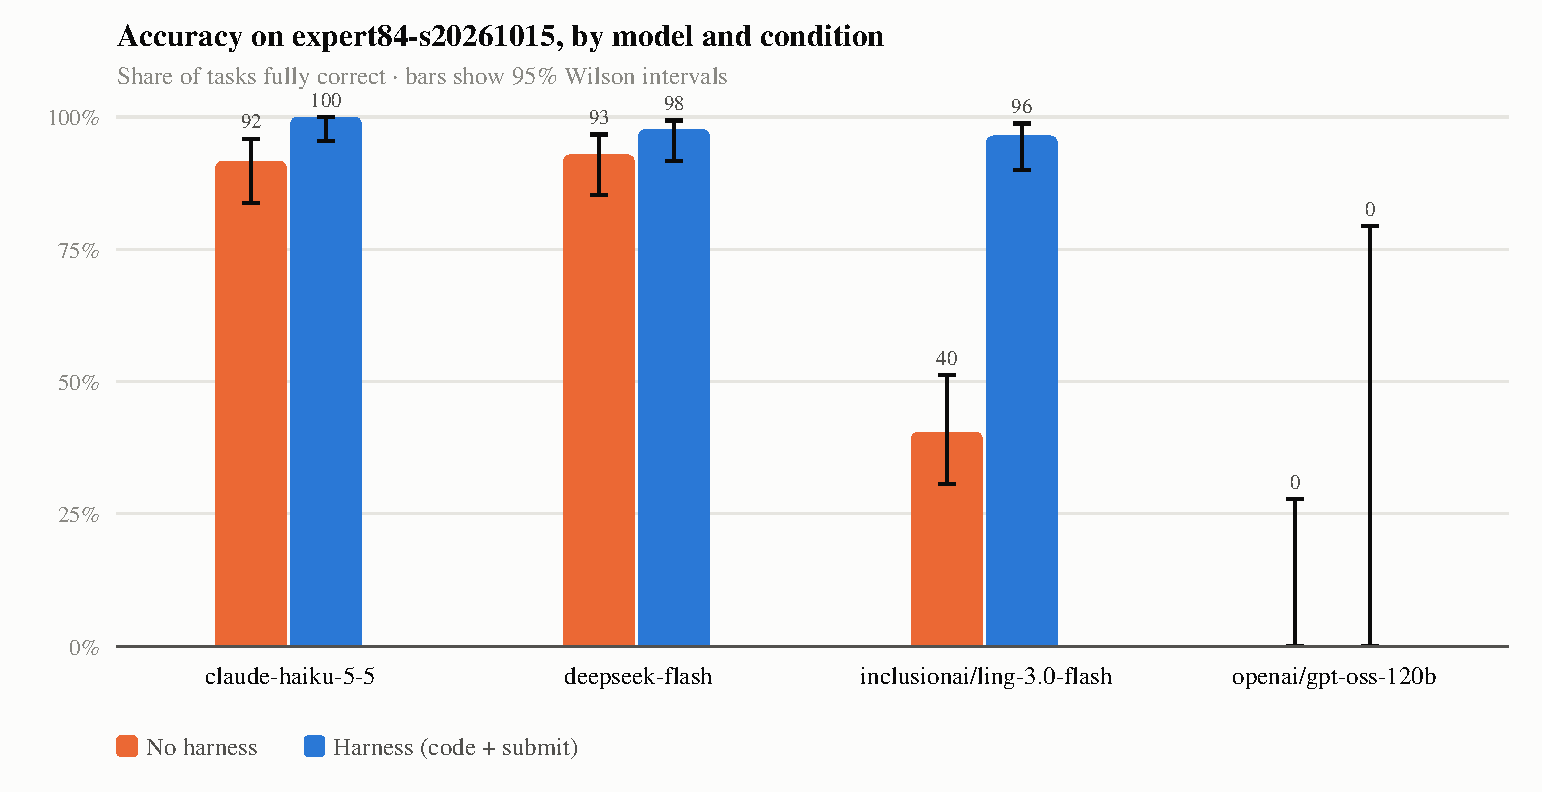
\includegraphics[width=.82\linewidth]{fig/fig_accuracy_expert84-s20261015.pdf}
\caption{Accuracy on expert84 by model and condition (bars: 95\% Wilson intervals). The gpt-oss-120b bars are not accuracy: it completed only 10 of 84 tasks without tools and 1 with them (timeouts), so no accuracy is claimed.}
\end{figure}

\subsection{What the lift is made of}
For ling, 40 of 50 baseline misses were no answer (32 out of tokens while reasoning in text, 8 unparseable); 10 were wrong values (7 off by more than 1\%, 3 near misses). Format compliance at baseline was 52.4\%. DeepSeek's baseline failures were 5 out-of-tokens and 1 unparseable, all in \texttt{wip\_portfolio}, with no numeric errors; the harness removed them but added 2 numeric errors on \texttt{mass\_haul}. Haiku's baseline had 4 numeric errors and 3 out-of-tokens, all removed. The 32{,}000-token cap was our setting (DeepSeek advertises 393{,}216), so a higher-cap baseline might recover some of the misses; this is untested.

\subsection{Efficiency reverses with task length}
On expert84 the harness cut output tokens by 63\% for Haiku (6{,}142 to 2{,}280) and 57\% for DeepSeek (13{,}960 to 6{,}069), and cost per correct answer from \$0.0036 to \$0.0019 (Haiku) and \$0.0034 to \$0.0011 (ling). On quick and fresh the harness raised cost. Tool overhead dominates short tasks; the baseline's own reasoning dominates long ones.
\begin{figure}[h]
\centering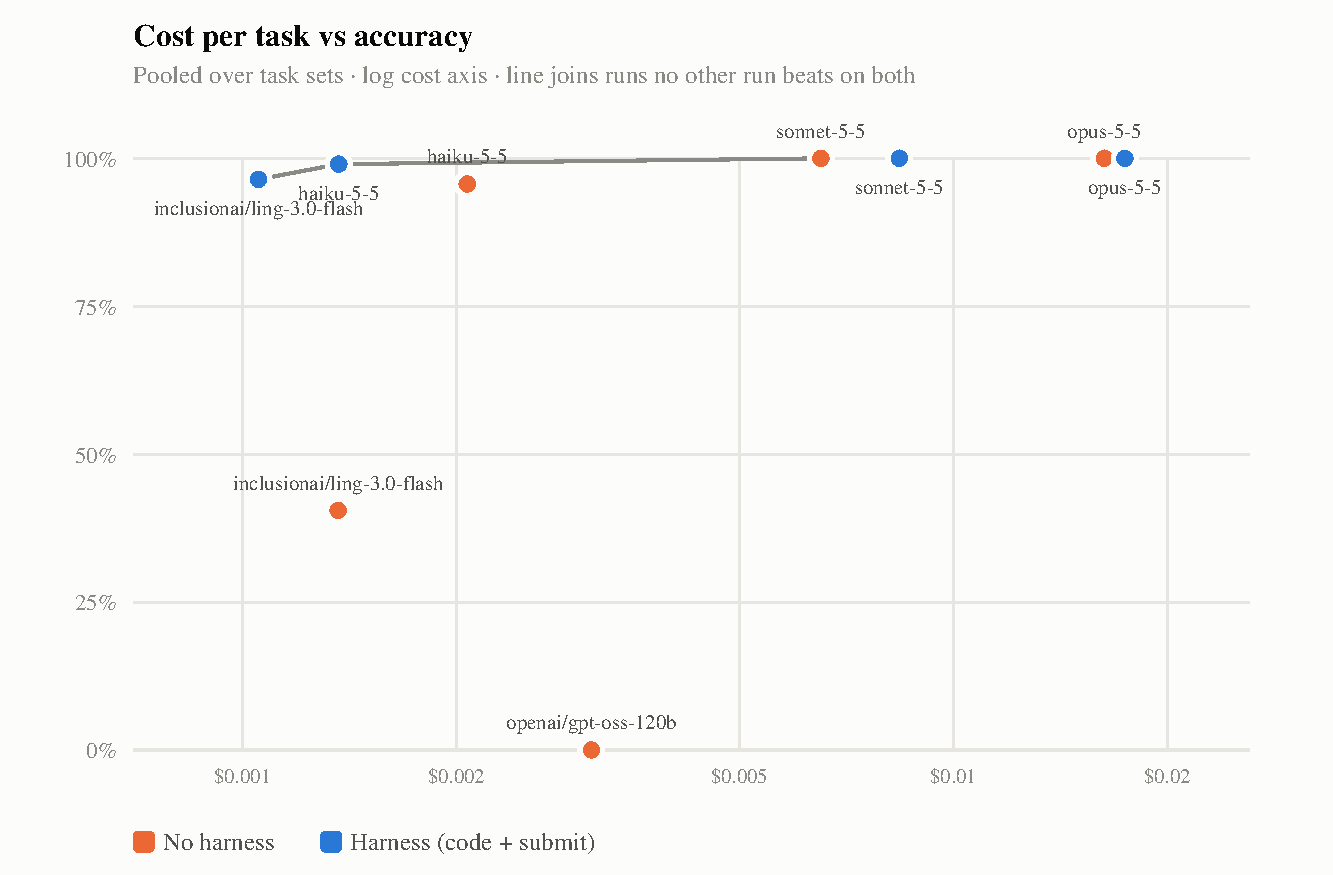
\includegraphics[width=.72\linewidth]{fig/fig_pareto.pdf}
\caption{Cost per task against accuracy, pooled over task sets (log cost axis; the line joins runs that no other run beats on both). Pooling mixes easy and expert sets, so use it for cost shape, not for ranking models.}
\end{figure}

\subsection{Making the benchmark harder: a success and a failure}
A calibration over expert84 and eight result files gave informativeness (mean $p(1-p)$) of 0.111 against 0.25 ideal, with 29 of 84 items passed by every run, 28 of them from three families whose rules are explicit and independent. We added a second level to each family and measured ling without tools, 12 items per cell:
\begin{table}[h]
\centering\small
\begin{tabular}{@{}lccc@{}}
\toprule
Family & First level & Second level & Change\\
\midrule
\texttt{pay\_app\_certification} & 11/12 (91.7\%) & 3/12 (25.0\%) & $-66.7$\\
\texttt{delay\_tia} & 10/12 (83.3\%) & 5/12 (41.7\%) & $-41.7$\\
\texttt{bid\_leveling\_expert} & 9/12 (75.0\%) & 12/12 (100\%) & $+25.0$\\
\bottomrule
\end{tabular}
\caption{Second-level families, ling-3.0-flash, no tools.}
\end{table}
Two second levels work: interacting rules (a stored-materials exclusion that the arithmetic-error rule never flags; a per-month weather allowance with two notice periods and two caps) cost fields rather than whole items. The third failed: adding rules made \texttt{bid\_leveling} more structured and therefore easier, so it is withheld from any v2 tier until redesigned. Difficulty comes from interacting conventions and reading traps, not from more explicit rules or volume, and each claimed escalation needs its own measurement. Caveat: $n=12$, one model, and the families were chosen using ling's failures. On the combined hard set (36 tasks) ling goes from 55.6\% (20/36) to 77.8\% (28/36), +22.2 points (CI +2.8 to +41.7; 12 better, 4 worse; $p=0.077$, not significant at 5\%).

\section{Methodological findings}\label{sec:method-findings}
\begin{enumerate}
\item \textbf{Two implementations.} Re-deriving answers from the prompt text caught a genuine design flaw (a rejected bid chosen from the naive ranking did not always change the winner) that the generator's own tests missed.
\item \textbf{Hunting for traps with conjunctive retries is not a design.} Traps are now built from the ranking a rule-ignoring model actually sees and asserted present in every item.
\item \textbf{A development seed makes a ceiling look like skill.} Quick overlaps harness development; fresh seeds were created after the harness was frozen.
\item \textbf{Report completion, format and accuracy separately.} An early summary counted API failures as wrong (ling's harness read 41.7\% when the truth on received answers was 97.2\%); gpt-oss-120b wrote correct values with no \texttt{ANSWER:} line and scored 0. Not-run tasks are now excluded from accuracy and shown separately, and a lenient score is shown beside the strict one, never instead.
\end{enumerate}

\section{Threats to validity}
\begin{itemize}
\item \textbf{Authors built both tasks and harness.} The expert tier came from an uninspected seed but was designed alongside the harness; toolkit functions exist because families need them.
\item \textbf{Second-level families were chosen using ling's failures}, so they are harder for that model than a neutral draw.
\item \textbf{Single run per task} on all headline results; repeats infrastructure exists but the three-repeat arm has not been run.
\item \textbf{Not effort-controlled} for OpenAI-compatible APIs (server default).
\item \textbf{Frontier models untested on the expert and extreme tiers} (budget). Claude spend was \$4.9986 of a \$5 cap.
\item \textbf{Text only.} Image families are excluded, so nothing here concerns drawing or plan reading.
\item \textbf{Exclusions.} gpt-oss-120b is excluded (10 of 84 and 1 of 84 completed).
\item \textbf{Harness flaw uncorrected.} The identifier-list schema issue is documented, not fixed, to avoid tuning after seeing results.
\item \textbf{Not our product.} The harness is the benchmark's sandbox, not the shipped assistant's tools, and no result here concerns a model we trained. The finding supports the approach, not the shipped build.
\end{itemize}

\section{Conclusion}
On long, interacting construction calculations, giving a model a calculator and a strict answer schema is worth more than model size: a cheap open-weight model moves from 40.5\% to 96.4\% and lands within a few points of mid-size and frontier-lab small models, at about a third of the cost per correct answer. On easy tasks, frontier models do not need the help and the harness only changes cost. Most of the open-weight gain is finishing inside the token budget, which is itself a practical result for anyone deploying small models. The honest limits are single runs, frontier models unmeasured on the expert tier, and authors who built both tasks and harness.

\section*{Remaining work before submission}
\begin{enumerate}[leftmargin=*]
\item Run the unread extreme (32) and rules-chain (24) sets for at least one cheap model per arm.
\item Run Opus and Sonnet on expert84 (planned cost about \$8 and \$20), or state that they are out of scope.
\item A labelled harness v2 (identifier-list fix) on every arm, per the decision rules.
\item A higher-token-cap baseline for ling and DeepSeek, to separate ``cannot calculate'' from ``ran out of budget''.
\item Three repeats on Haiku and one open-weight model to measure run-to-run variance.
\item Redesign \texttt{bid\_leveling\_expert\_hard}; run the project's own fine-tuned small model through both conditions; reconcile client-side Claude cost against the invoice; archive the result files and decide what to publish and under what licence.
\end{enumerate}
\end{document}
